\section{The \textit{Minecraft} Water Problem}

% put an intro here
\noindent Our problem uses the popular game \textit{Minecraft} and its properties as its base. In \textit{Minecraft}, the player can generate a "random" world, in which he can then place and break blocks at will. For the \textit{Minecraft Water Problem} we took an abstract version of \textit{Minecraft}, using the natural mechanics of the game and setting certain rules for world generation and updates of the world (Ticks). In the further sections of this paper, we will discuss the required rules to make our problem possible and a detailed description of why this problem is NP-Complete.

\subsection{The World} 

\noindent A \textit{Minecraft} world is an arrangement of blocks, which each have three coordinates to refer to their position and a block name to specify the properties of the block. For our specification, the \textit{Minecraft} world is seen as a 3D-Array, where every field has the block from this position in the world or contains nothing (in \textit{Minecraft} this would be the air block). 

\noindent For our problem we check if a certain \textit{Minecraft} world meets the criteria of \textbf{MCWATER}. The world needs to satisfy the following rules: 

\begin{itemize}
    \item It can only contain certain blocks (specified in section \ref{blocks})
    \item The player may not change anything in the world
    \item Special rules for interaction of blocks (specified in section \ref{blocks})
\end{itemize}

\subsection{Allowed Blocks in \textbf{MCWATER}} \label{blocks}

\noindent For our definition of the \textit{Minecraft Water Problem}, we limit the usage of blocks/objects that we can place in our world to the following 7:
\newline \textit{(Every block except string, sand and water can be replaced by almost every "normal" building block from the game, since they serve no functionality. We simply chose these blocks for color differentiation!)}
\paragraph{Wool\cite{minecraftfandom:wool}}
Wool is a block that can be obtained from sheep in the game.
They can be colored in 16 different colors with the corresponding dye.
For our problem, we use wool to indicate a path or a channel through which water can flow.
We will use five different colors with different definitions:
\begin{itemize}
    \item White wool: path of a variable
    \item Light gray wool: path of the negation of the variable
    \item Orange wool: transitional path between the two former
    \item Magenta wool: part of the splitter (later described in Section \ref{splitter})
    \item Cyan wool: part of the collector (later described in Section \ref{collector})
\end{itemize}

\paragraph{Glass\cite{minecraftfandom:glass}}
Glass is a block that can be obtained by smelting sand in a furnace.
We use it as the borders for the paths through which water can flow.

\paragraph{Block of Gold\cite{minecraftfandom:bog}}
A Block of Gold can be obtained by crafting nine gold ores together.
\newline It shows whether an assignment is satisfiable or not depending on whether all gold blocks in the world are covered by water.

\paragraph{Block of Lapis Lazuli\cite{minecraftfandom:boll}}
A Block of Lapis Lazuli can be obtained by crafting 9 Lapis Lazuli minerals together.
They mark the position of the water source that represents the variables.

\paragraph{String/Tripwire\cite{minecraftfandom:string}}
A piece of string can be obtained by defeating a spider in the game.
They can be placed on top of blocks or in the air and interact with objects and are now called a tripwire.
The property most relevant to our problem is that if a tripwire is below a block that could fall due to gravity, the block will not fall.
We will use this to prevent a sand block from falling.
Tripwires will be destroyed if water is flowing to the same coordinate.

\paragraph{Sand\cite{minecraftfandom:sand}}
Sand is a block that is generated near water or in a desert biome.
It is one of the few blocks in \textit{Minecraft} that is influenced by gravity.
\marginpar{\tiny If there are no blocks at all below sand, then we assume it just gets deleted from the world.}{If} there is no solid block or string below the sand, it will fall until it cannot go any further.
We use this property to prevent water from flowing into an unwanted channel. In the game, there is some delay between falling and being placed again, but for the definition of our problem, we say the sand will fall one step every tick.

\noindent \newline For example, if a string is below a sand block, it will not fall, but if the string is destroyed, the sand will take its place by falling one block below.

\paragraph{Water}
Water naturally generates in the world to form oceans, rivers, and springs\cite{minecraftfandom:water}. 
It mimics the properties of water(as a fluid) in the real world.
We differentiate water into two types, the source block and flowing water, which can have 7 different water levels that will be explained in \ref{waterflow}. 
If there are no air blocks (or simply empty blocks) in the adjacent tiles,
the water stands still. Otherwise the water spreads according to a specific flow logic.

\paragraph{Flow behavior of water} \label{waterflow}
Water spreads horizontally and downward into nearby air. When a water block is placed, it always checks the surrounding 5 by 5 area for air blocks one level below the water, so it can flow there directly. If an air block is found, the water will spread directly into this air block, if not the water will continue its natural flow in each possible horizontal direction for 7 blocks. Every time the water spreads one block in a direction it performs the before mentioned 5 by 5 scan for holes to flow into. The maximum a single water block can spread is shown in Figure \ref{fig:normalflow}.

\begin{figure}[ht]
  \centering
  \begin{minipage}[b]{0.4\textwidth}
    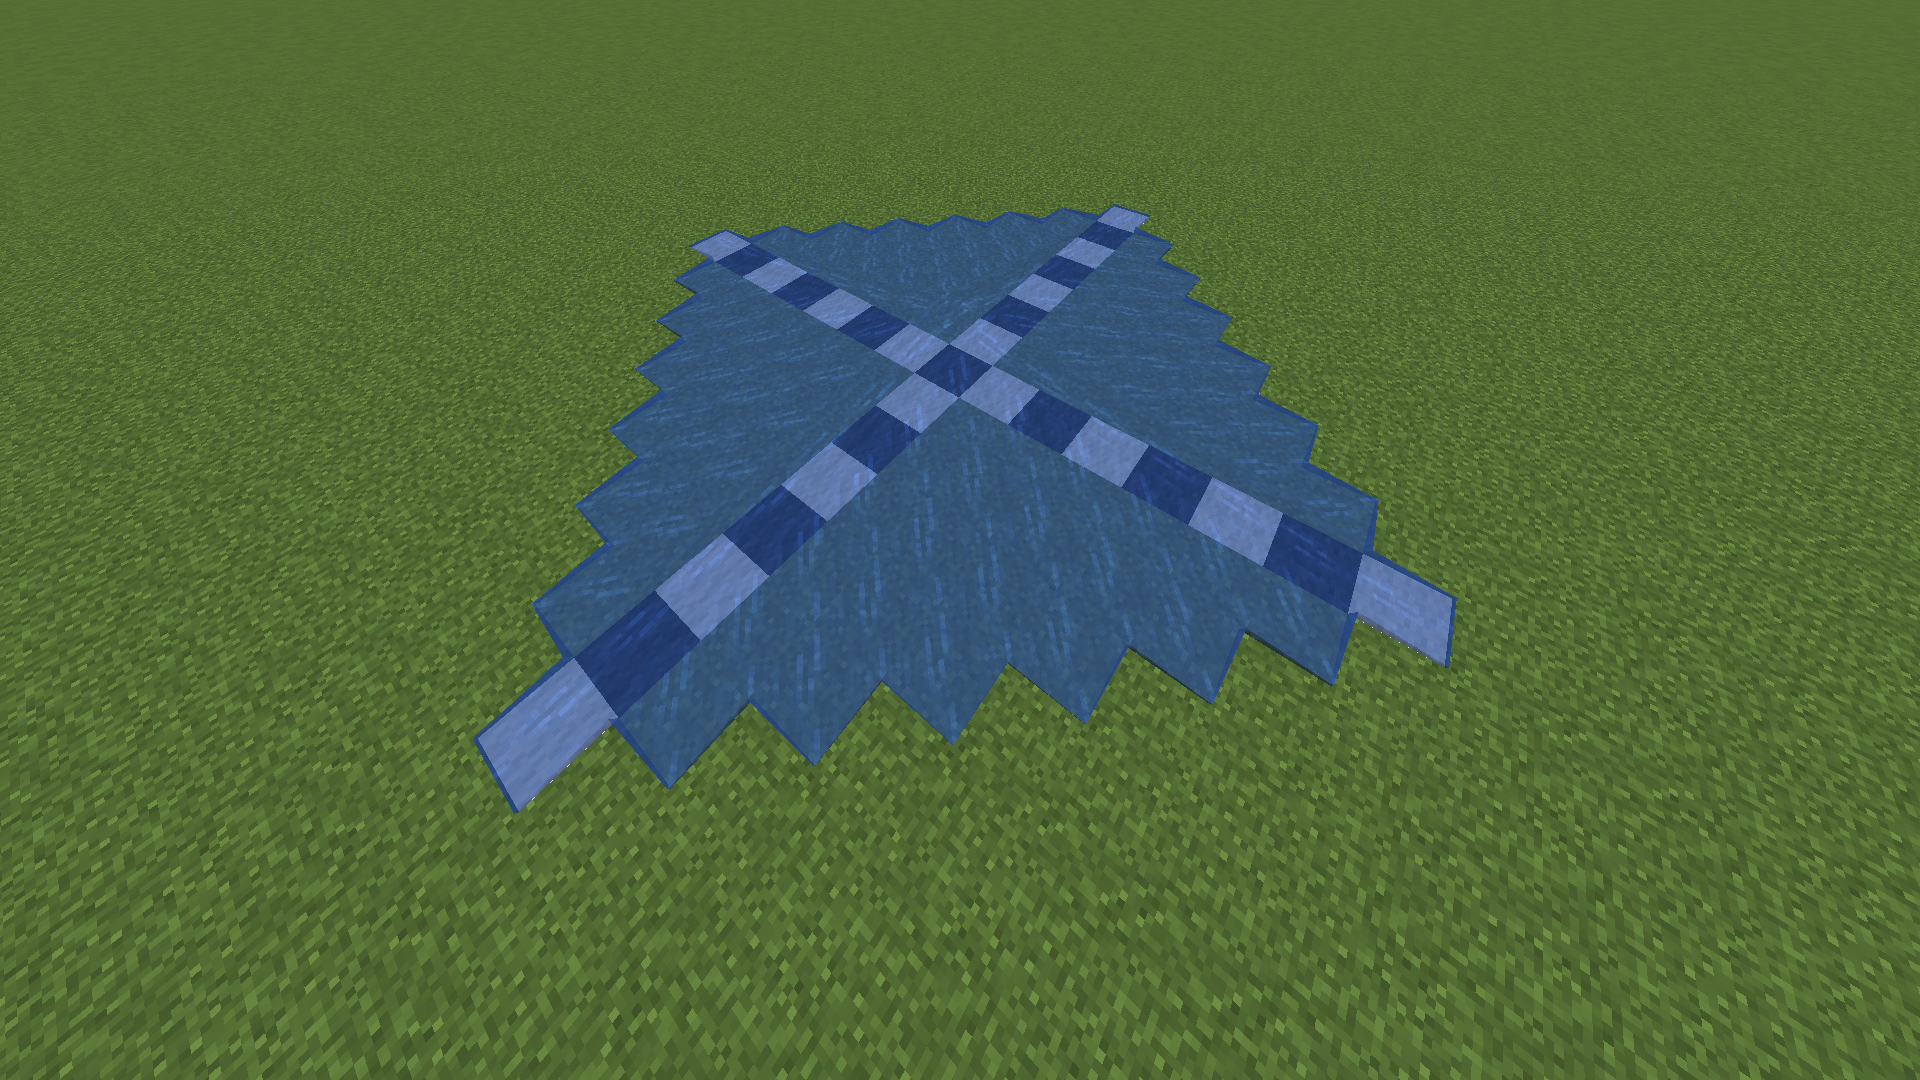
\includegraphics[width=\textwidth]{images/waterflownoair.png}
    \caption{Normal water flow}
    \label{fig:normalflow}
  \end{minipage}
  \hfill
  \begin{minipage}[b]{0.4\textwidth}
    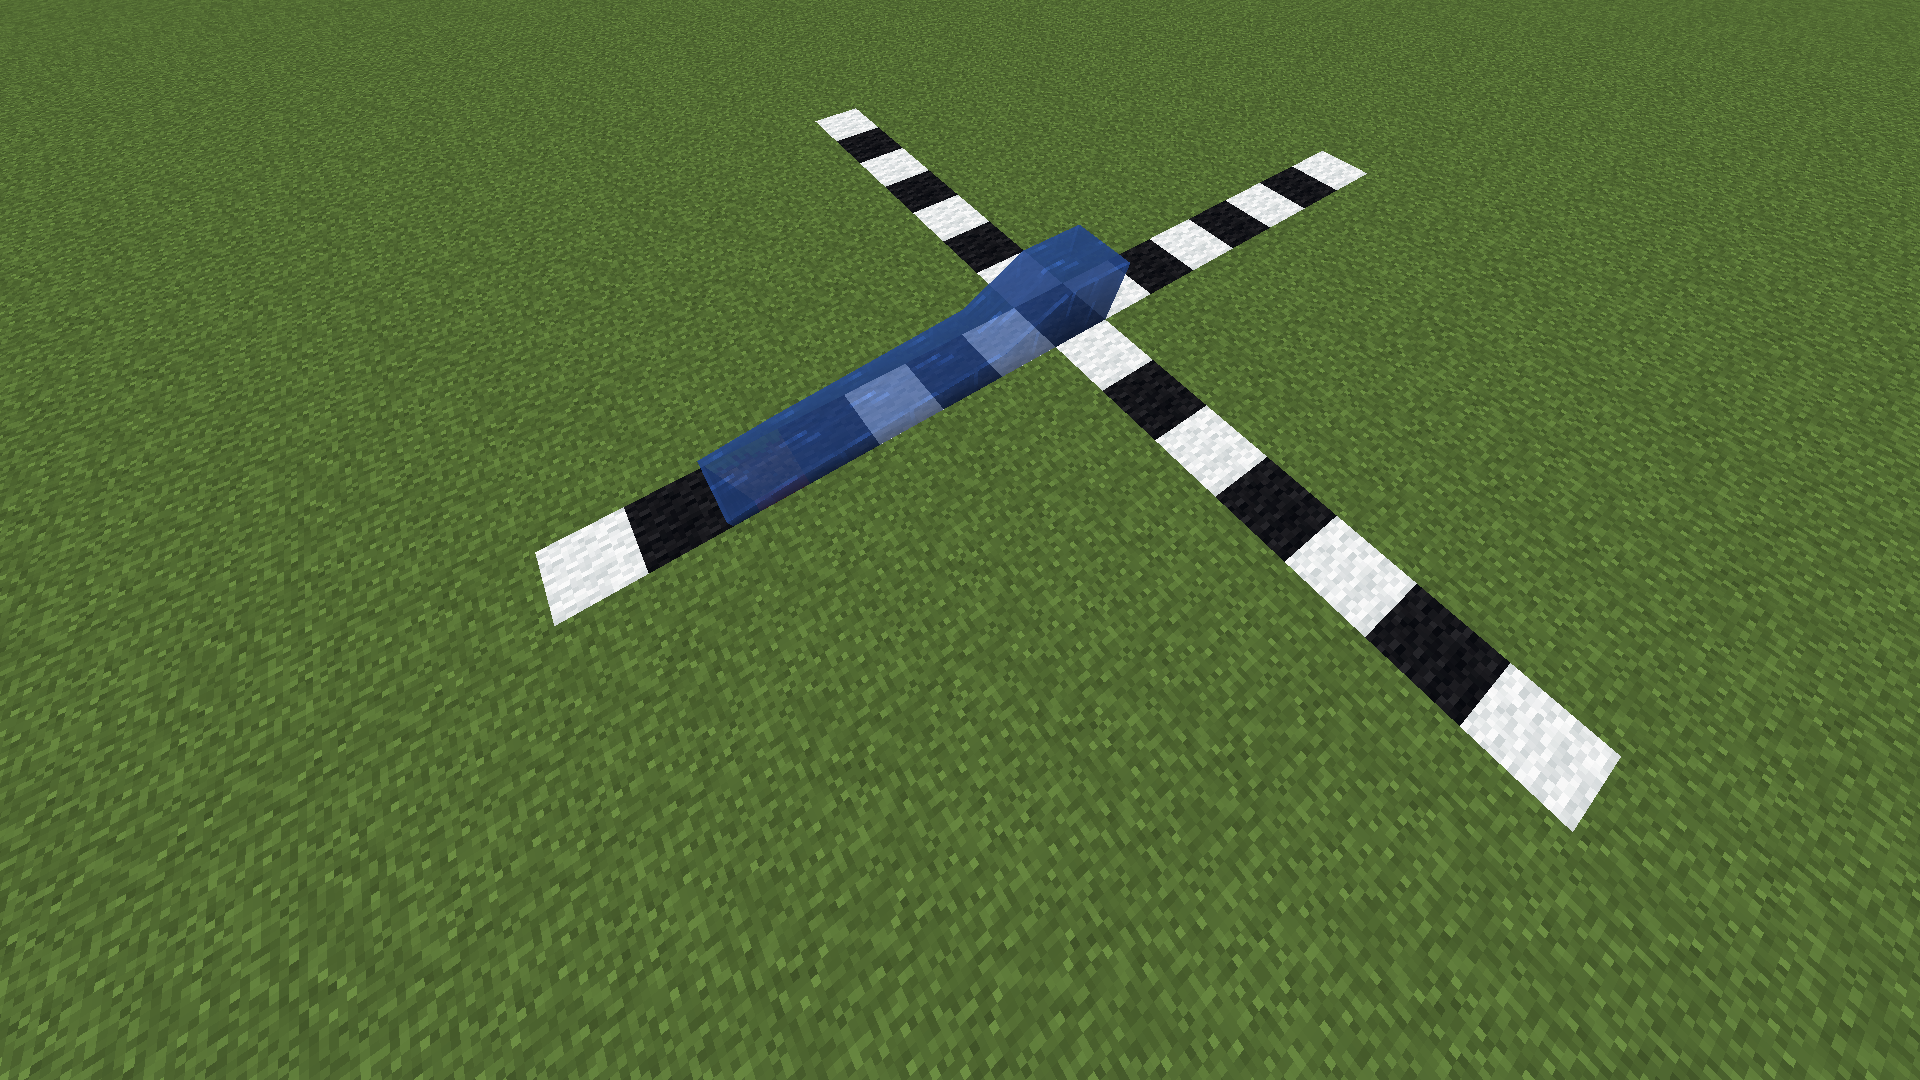
\includegraphics[width=\textwidth]{images/waterflowhole.png}
    \caption{Water flowing to hole}
    \label{fig:holeflow}
  \end{minipage}
\end{figure}
\pagebreak


\marginpar{\tiny When water flows infinitely out of the world, we can assume it disappears because it does not change the outcome of the problem.} \noindent Water can spread downward infinitely until stopped by a block. Water spreads at a rate of 1 block every 5 game ticks, or 4 blocks per second \cite{minecraftfandom:waterspread}.

\noindent This definition refers to the actual in-game tick system, however we use our own abstraction described in section \ref{blockupdates}.
Therefore we summarize 5 game ticks to a single block update.
\newline If there is a need to extend the water flow, we can move the flow one layer (or block) below in the 7 block range from the source block.
The value that is used to determine the current flow is reset and we have another 7 blocks to work with that can also be extended as needed.
\newline When water flow gets blocked by a solid block, the water after the block gets drained, or simply: it disappears. In the game, this does not happen instantaneously, but to simplify the definition we assume it does at a block update.

\begin{figure}[h]
    \centering
    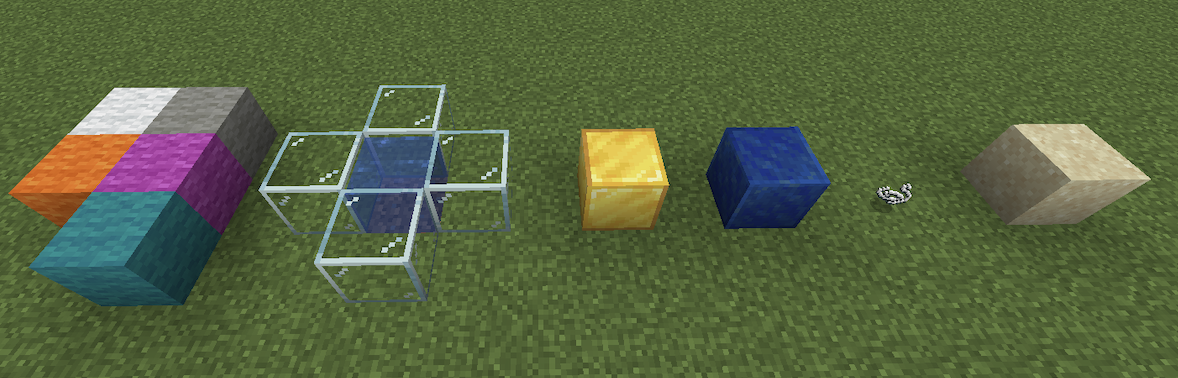
\includegraphics[width=\linewidth]{images/allowed blocks.png}
    \caption{allowed blocks as described from left to right (water encased in glass)}
    \label{fig:allowedblocks}
\end{figure}


\vspace{2cm}

\subsection{Block Updates} \label{blockupdates}
\noindent In \textit{Minecraft}, the "chunks" (chunk = 16 by 16 area of the world) that are currently loaded in the memory are updated in "ticks". The dynamics behind these ticks and which blocks are affected are complicated, which is why we will not dive deeper into this subject. For our problem we say that every chunk is always loaded, otherwise parts of the world could not receive block updates. There will be a deeper explanation about the updating of blocks in section \ref{updating} \textit{Updating the World}, but we will go over the basics. 

\noindent Firstly, we need to set rules which will help in the following explanation:

\begin{itemize}
    \item If a block wants to replace water, it will always do so
    \item When water wants to replace a tripwire, it will always do so
    \item If two water blocks meet, the one with the higher water level will win \textit{(Water level is described in \ref{waterflow})}
    \item If two flowing waters at the highest water level meet, they will form a solid water block.
\end{itemize}

\noindent When performing a block update, we go through every block and ask them how they want to change their environment. When a block wants to make changes to another block it will overwrite that block as an "update block" which shows that this block has been updated in the current tick and does not need to be updated in this tick. If another block wants to change an already updated block, we will check the rules and change that block accordingly. 

\noindent It is also important to note that the number of blocks that are taken into account in each update is always constant.

\subsection{Definition}

Now that the cornerstones of our problem are defined we can give a formal definition of our Language \textit{WATERGOLD}:

\noindent A \textbf{MCWATER} world is part of \textit{WATERGOLD} if there exists a subset of lapis lazuli Blocks, so that every gold block is covered by water if we place a water block on every lapis lazuli Block of this subset at the same time. For this check, we will update the \textbf{MCWATER} world until no changes are made anymore.

